\documentclass{article}
\usepackage[utf8]{inputenc}
\usepackage[T1]{fontenc}
\usepackage{ngerman}
\usepackage{graphics}
\usepackage{pdfpages} 
 
\title{User-Centered Design\\~\\Projektbericht\\ \small{T. Bento, N. Lehmann, B. Swiers}}
\date{10.05.2015}

\renewcommand{\contentsname}{Inhaltsverzeichnis}

\begin{document}
\renewcommand\abstractname{UR.S.U.L.A. (yoUR Study and Universial Learning Assistent)}
\maketitle

\includegraphics{img/title_pic.jpg}
\begin{abstract}
{\huge L}ernverwaltungssoftware der nächsten Generation, UR.S.U.L.A.!\\
\end{abstract}

\newpage

\tableofcontents

\newpage

\section{Zusammenfassung}

Dieses Dokument stellt einen Arbeitsreport für die Entwicklung einer Lernverwaltungssoftware (LMS) unter Verwendung von Techniken der benutzerzentrierten Softwareentwicklung dar.\\
\\
Es zeigt den Entwicklungsprozess von der Ermittlung der Benutzerbedürfnisse bis hin zur Gestaltung der Benutzeroberfläche. Für diesen Zweck wird ein Modell von Jesse James Garret mit Anpassungen durch Frau Prof. Dr. C. Müller-Birn verwendet, dass den Ablauf in fünf Phasen aufgliedert. Es werden alle Zwischenschritte dokumentiert und die Vorgehensweise bei den jeweiligen Arbeitsschritten erläutert.\\
\\
Das zentrale Element der Untersuchung ist die Usability des entstehenden Produkts. Der Begriff \textit{Usability} definiert sich nach ISO 9214-11 dadurch, dass \textit{spezifizierte Nutzer} effektiv, effizient und befriedigend \textit{spezifizierte Ziele} erreichen und das in einem \textit{spezifizierten Kontext}. Nielson hingegen definiert Usability als Qualitätsmerkmal, das durch die Erlernbarkeit, Effizienz, Einprägsamkeit, Fehleranfälligkeit in der Benutzung und Zufriedenheit determiniert wird.

\newpage

\section{Einleitung}

\subsection{Motivation / Projekthintergrund}

Das Ziel dieses Projektes ist die Entwicklung eines Lernverwaltungssystems für die Freie Universität Berlin.
Es soll eine Software geschaffen werden, die den Alltag an der Universität erleichtert und die elementaren Arbeitsprozesse von Lehrenden, Studierenden, wissenschaftlichen Mitarbeitern und Verwaltungsangestellten vereinfacht und optimiert.
Da die derzeit verwendeten Systeme den Bedürfnissen der Nutzer nicht gerecht werden, entstand der Wunsch nach einem zentralen System, welches sich möglichst einfach bedienen lässt und alle für die Benutzer benötigten Funktionalitäten in einem System vereint. 

\subsection{Struktur dieses Dokuments}

\begin{itemize}
\item Im Teil \textit{Projektablauf} wird die prinzipielle Vorgehensweise in diesem Projekt beschrieben. Anders als in einem regulären Projekt strukturieren wir den Ablauf anhand eines neuen Modells.
\item Im Teil \textit{Goals / Ziele} wird das Sammeln von Informationen, vom Konzipieren geeigneter Interviewfragen bis hin zu der Auswertung der Interviewergebnisse beschrieben.
\item Im Teil \textit{Scope / Umfang} wird die weitergehende Analyse beschrieben. Thematisiert werden unter anderem die Benutzergruppen, die Persona und das Szenario.
\item Im Teil \textit{Structure / Struktur} wird ebenfalls weitergehende Analyse beschrieben. Es werden Primärsubstantive herausgearbeitet, um einen Aufgabenstrom zu identifizieren der anschließend mit Hilfe von einem Flowchart abgebildet wird.
\item Im Teil \textit{Skeleton/Skelett} wird der resultierende Paperprototype und die mit diesem durchgeführten Testmethoden und Tests beschrieben.
\item Im Teil \textit{Surface / Oberfläche} wird die Verbesserung des Paperprototypes mit Hilfe der heuristischen Evaluation beschrieben sowie die Umsetzung in einen high fidelity prototype.
\end{itemize}

\newpage

\section{Projektablauf}

Das hier beschriebene Projekt findet im Kontext der Lehrveranstaltung \textit{User Centered Design} statt und hat daher ein geringfügig anderen Charakter als ein reguläres Projekt, da der Benutzer das treibende Entscheidungskriterium während des gesamten Prozesses darstellt. Im Gegensatz zu einem regulären Projektablauf, werden wir dieses Projekt nicht in die Phasen Analyse, Modellierung, Implementierung und Testen gliedern, sondern uns am Modell von Jesse James Garret mit den Änderungen und Ergänzungen von Dr. C. Müller-Birn orientieren.

\newpage

\section{Goals / Ziele}

Dieser Teil beschäftigt sich mit der Datengewinnung und -auswertung. Wir haben uns für eine direkte Untersuchungsmethode mit Individuen entschieden: das Interview. Diese Methode adressiert die beiden Bereiche Inhalt und Anwendung.

\subsection{Interviews}

Das Produkt \textit{UR.S.U.L.A.} richtet sich prinzipiell an alle Beteiligten des universitären Lehr- und Lernprozesses. Aus Gründen der Durchführbarkeit dieses Projekts haben wir uns im Folgenden jedoch auf die Zielgruppe \textit{Studierende} fokussiert.\\
\\
Das Ziel der Analyse ist es herauszufinden welche Anforderungen und Bedürfnisse die Nutzer der Software haben, wobei auch versucht wird das Verhalten der Nutzer zu erfassen.\\
\\
Es standen uns prinzipiell drei Methoden zum Erfassen von Benutzerinformationen zur Verfügung:
\begin{itemize}
\item Interviews
\item Beobachtungen der Nutzer
\item Kontextanfragen
\end{itemize}
Wir haben uns für Interviews entschieden, da wir diese Methode notfalls später auch gut mit anderen Methoden kombinieren können.\\
\\
\underline{Die für uns relevanten Informationen beziehen sich auf}:
\begin{itemize}
\item Benutzer
	\begin{itemize}
	\item mentales Modell des Benutzers
	\item Ziele und Motivation des Benutzers
	\item implizite Annahmen des Benutzers
	\item präzise Informationen über die Aufgaben des Benutzers
	\item benutzerrelevantes Domainenwissen
	\end{itemize}
\item Produkt
	\begin{itemize}
	\item Verwendungskontext
	\item Wie kann der Benutzer bei seinen Aufgaben unterstützt werden?
	\item Probleme mit dem aktuellen Produkt
	\end{itemize}
\end{itemize}

\newpage

\subsection{Konzipierung}

Bevor wir den Interviewleitfaden erstellt haben, haben wir einige Fragen formuliert und mit dem Fokus auf Verständlichkeit an einer kleinen Testgruppe getestet. Dabei stellte sich heraus, dass wir einige Änderungen vornehmen sollten:
\begin{itemize}
\item Wir haben die Anrede von der Sie-Form zur Du-Form geändert, um einen persönlicheren Kontakt zur Zielgruppe zu erlangen.
\item Wir haben alle geschlossenen Fragen eliminiert und in offene Fragen transformiert.
\item Wir haben Fachbegriffe und Abkürzungen eliminiert, die unverständlich sein könnten, bzw. geändert in verständliche Sprache.
\end{itemize}
Aus der Korrektur der Fragen ergab sich folgender Interviewleitfaden:
\begin{enumerate}
\item Welches Fach studierst Du und warum?
\item Wie sieht Dein Alltag an einem gewöhnlichen Universitätstag aus?
\item Welche Lernverwaltungssoftware der Freien Universität Berlin hast Du schon einmal verwendet?
\item Wann und wo verwendest Du die Lernverwaltungssoftware der Freien Universität Berlin?
\item Wie zufrieden bist Du im Allgemeinen mit der derzeitigen Lernverwaltungssoftware der Freien Universität Berlin und warum?
\item Welche Funktionen der Lernverwaltungssoftware verwendest Du wirklich?
\item Wie zufrieden bist Du mit den genannten Funktionen und warum?
\item Was würdest Du anders machen?
\item Verwendest Du zum Erreichen Deiner studienbezogenen Ziele auch andere Softwaresysteme oder Webseiten, etc.? Wenn ja, welche und warum?
\item Auf welchen Endgeräten verwendest Du die von Dir bevorzugte Software, Webseiten, etc.?
\item Welche Probleme während Deines derzeitigen Studienalltags werden durch Software nicht gelöst oder können Deiner Meinung nach nicht von Software gelöst werden?
\item Wer unterstützt Dich während Deines Studiums und wie?
\item Wenn Du eine Empfehlung zu einem Modul oder einer Lehrveranstaltung erhältst, was sind für Dich die wichtigsten Punkte?
\item Wie schätzt Du Deine Studienleistungen ein und warum?
\end{enumerate}

\subsection{Durchführung}

Wir haben uns einen Raum (Medienraum K40 in der Takustr. 9, 14195 Berlin) gebucht und 8 Personen (4 männliche und 4 weibliche Studierende der Informatik) zu einem Interviewgespräch persönlich eingeladen. Von den 8 eingeladenen Personen erschienen 6 Personen. Alle Gespräche wurden mit einem Aufnahmegerät (Mobiltelefon) aufgezeichnet. Um eine angenehme Interviewatmosphäre herzustellen begannen wir jedes Interview mit einer ca. 3 minütigen Warmup-Phase. Im Anschluss folgte das Interview entlang des Leitfadens mit geringen Abweichungen, je nach Gesprächspartner. Nach den Interviewgesprächen wurden die Aufnahmen verschriftlicht und ausgewertet.

\subsection{Ergebnisse}

\begin{enumerate}
\item Welches Fach studierst Du und warum?
\begin{itemize}
\item Informatik, weil er/sie nicht wusste, was er/sie nach dem Abitur tun sollte
\item Bioinformatik, weil reine Biologie zu langweilig ist und er/sie in die Forschung will
\end{itemize}

\item Wie sieht Dein Alltag an einem Universitätstag aus?
\begin{itemize}
\item Besuch der Vorlesung, Essen in der Mensa, Tutorium, mit Übungspartner treffen und Übungen bearbeiten, zu Hause Übungsaufgaben lösen
\item Zeit in der Universität: durchschnittlich 10 bis 18 Uhr
\end{itemize}

\item Welche Lernverwaltungssoftware der Freien Universität Berlin hast Du schon einmal verwendet?
\begin{itemize}
\item KVV / Sakai CLE
\item Campus Management (nur zur Modulbuchung)
\end{itemize}

\item Wann und wo verwendest Du die Lernverwaltungssoftware der Freien Universität Berlin?
\begin{itemize}
\item in der Universität:
	\begin{itemize}
	\item zur Bearbeitung eines Übungszettels
	\item für Skripte in einer Vorlesung (Skript, wird nicht gespeichert)
	\item zur Modulbuchung am Anfang des Semesters
	\end{itemize} 
\item zu Hause:
	\begin{itemize}
	\item zur Bearbeitung eines Übungszettels
	\item zur Modulbuchung am Anfang des Semesters
	\end{itemize}
\item unterwegs:
	\begin{itemize}
	\item Ankündigungen abrufen
	\item Neuigkeiten lesen
	\end{itemize}
\end{itemize}

\item Wie zufrieden bist Du im Allgemeinen mit der derzeitigen Lernverwaltungssoftware der Freien Universität Berlin und warum?
\begin{itemize}
\item Negative Aspekte:
	\begin{itemize}
	\item es gibt zu viele verschiedene Systeme, besser wäre ein System
	\item man muss sich immer wieder neu einloggen, da man nach einiger Zeit automatisch ausgeloggt wird
	\item Übersetzung Deutsch/Englisch ist schlecht
	\item Benutzer von Apple-Produkten haben Probleme mit den Systemen
	\item es werden keine Inhalte auf Endgeräte synchronisiert
	\end{itemize}
\item Positive Aspekte:
	\begin{itemize}
	\item einfach zu bedienen (bspw. Anmeldung zu einem Tutorium)
	\item übersichtlich, man findet was man sucht
	\item gut nach Fächern strukturiert
	\item man wird per Email informiert
	\end{itemize}
\end{itemize}

\item Welche Funktionen der Lernverwaltungssoftware verwendest Du wirklich?
\begin{itemize}
\item Anmeldung zu Modulen / Lehrveranstaltungen
\item Übungszettel ansehen/herunterladen
\item Übungszettel abgeben/hochladen
\item Anmeldung zu einem Tutorium
\item Skripte/Folien/Materialien ansehen/herunterladen
\item Ankündigungen lesen
\item Forum (inhaltliche und organisatorische Fragen stellen)
\item Punkte/Noten einsehen
\item Herausfinden wo mein Raum ist
\item Kalender
\end{itemize}

\item Wie zufrieden bist Du mit den genannten Funktionen und warum?
\begin{itemize}
\item Anmeldung zu Modulen / Lehrveranstaltungen: kompliziertes Zusammensuchen der Informationen in vielen verschiedenen Systemen; Man findet die Kurse nicht oder sie heißen anders, das ist schlecht!
\item Übungszettel ansehen/herunterladen: benachrichtigt werden ist gut, sehr zufrieden
\item Übungszettel abgeben/hochladen: einfach, man kann kommentieren, sehr zufrieden
\item Anmeldung zu einem Tutorium: sehr simpel, sehr gut
\item Skripte/Folien/Materialien ansehen/herunterladen: Ordnerstruktur ist sehr übersichtlich, aber ich hatte keine Möglichkeit den ganzen Ordner herunterzuladen oder zu synchronisieren
\item Ankündigungen lesen: benachrichtigt werden ist gut, sehr zufrieden
\item Forum (inhaltliche und organisatorische Fragen stellen): mit anderen Studenten in Kontakt kommen, es wurde immer geantwortet, ist gut strukturiert, positiv
\item Punkte/Noten einsehen: schlechte Übersicht, zu viele Klicks
\item Herausfinden wo mein Raum ist: unzufrieden, komplizierte Suche, kaum Softwareunterstützung
\item Kalender: unzufrieden, wenn ich mich in mein Tutorium anmelde, sollte das auch in meinem Kalender auftauchen, sollte mit anderen Kalendern synchronisierbar sein
\end{itemize}

\item Was würdest Du anders machen?
\begin{itemize}
\item Lernverwaltungs-App herausbringen, leichterer Zugriff
\item Ein System statt viele Systeme, sonst doppelte Arbeit.
\item die Übersetzung
\item Die meisten Probleme, die ich habe, sind nicht durch Software lösbar.
\item das Suchproblem (Module/Lehrveranstaltungen) ändern/lösen.
\item Resources-Ordner sollte downloadbar/synchronisierbar sein
\item Home-Übersicht erschlagend, hier braucht man nur: Kalender, Ankündigungen, aber keine Informationen über Bereiche
\end{itemize}

\item Verwendest Du zum Erreichen Deiner studienbezogenen Ziele auch andere Softwaresysteme oder Webseiten, etc.? Wenn ja, welche und warum?
\begin{itemize}
\item Youtube
\item Webseiten, die mit Videos einfach erklären, wie etwas funktioniert
\item MOOC (massiv online open courses)
\item Github / Gitlab
\item Wolfram Alpha
\item Wikipedia
\item Java Bibliothek
\item Galileo Open Books / kostenlose Softwarebücher im Internet
\item Mathematik- und Informatikforen
\item Latex
\item Microsoft Office / Open Office
\item in einer kleinen Gruppe Aufgaben durchsprechen ist wichtiger als Software
\end{itemize}

\item Auf welchen Endgeräten verwendest Du die von Ihnen bevorzugte Software?
\begin{itemize}
\item Laptop / Notebook
\item PC / Workstation
\item Smartphone
\item Tablets (nur Webseiten, sehr wenig genutzt)
\end{itemize}

\item Welche Probleme während Deines derzeitigen Studienalltags werden durch Software nicht gelöst oder können Deiner Meinung nach nicht von Software gelöst werden?
\begin{itemize}
\item Planung, Stundenplan, rechtzeitig eintragen
\item Leistungsdruck, bestimmte Regelung, wie viel man schaffen muss
\item Wo finde ich Inhalte?
\item Übungsaufgaben verstehen / Verständnisfragen
\item man braucht länger, um mit Software zu lernen, mit Menschen reden ist wichtiger
\item Schlafmangel ist wichtiger Faktor / einen guten Wochen-Rhythmus finden
\end{itemize}

\item Wer unterstützt Dich während Deines Studiums und wie?
\begin{itemize}
\item Lerngruppen! ...sich kennen lernen ist wichtig
\item Studierende aus höheren Semestern
\item Tutoren
\item Mentoren, wenn man Fragen hat wie man das Studium ausrichten soll
\item Motivation durch Freunde und Eltern
\end{itemize}

\item Wenn Du eine Empfehlung zu einem Modul oder einer Lehrveranstaltung erhalten, was sind für Dich die wichtigsten Punkte?
\begin{itemize}
\item muss ich es machen
\item Leistungspunkte
\item zeitlich, ob es in meinen Plan passt
\item interessiert es mich inhaltlich
\item Wer belegt noch die Lehrveranstaltung?
\item Es ist nicht so wichtig wie viele Leute mir etwas empfehlen, sondern wer.
\item Die Person, die mir das Modul empfiehlt, muss das Modul belegt haben.
\item Welcher Lehrende ist in der LV? (die Art wie man unterrichtet ist entscheidend)
\item Welcher Tutor ist in der LV? (die Art wie man unterrichtet ist entscheidend)
\item praktisch / theoretisch ist wichtig
\end{itemize}

\item Wie schätzt Du Deine Studienleistungen ein?
\begin{itemize}
\item Ich bin zufrieden mit mir.
\end{itemize}
\end{enumerate}

\subsection{Fazit}

\underline{Von uns identifizierte Funktionen sind}:
\begin{itemize}
\item Planung und Buchung von Lehrveranstaltungen
\item Empfehlungssystem für Lehrveranstaltungen
\item Lerngruppen finden
\item Synchronisierung von Lerninhalten
\item Mobile-KVV-Application für den Empfang von Nachrichten und Inhalten
\end{itemize}
Eine der wichtigsten Funktionen, die wir identifiziert haben, ist die Anmeldung zu Lehrveranstaltungen, bzw. Planung eines Semesters, die wir im weiteren Verlauf des Projektes aufgreifen und umsetzen wollen.

\newpage

\section{Scope / Umfang}

Mit den gewonnen Erkenntnissen aus den Interviews werden Benutzergruppen definiert und anschließend aus diesen eine Persona abgeleitet. Die Persona repräsentiert eine typischen Nutzer einer Benutzergruppe, gibt ihm ein Gesicht und ermöglicht es so sich besser in die Nutzer des Produktes hineinzuversetzen und das mentale Modell zu kommunizieren. Das Szenario, das den Umfang der Anforderungen erfasst und beschreibt was ein Nutzer tut wird erstellt. 

\subsection{Benutzergruppe}

Eine Benutzergruppe beschreibt abstrakt eine akkumulierte Menge von Benutzern. Wir haben folgende Benutzergruppen (mit der Einschränkung auf Studierende) identifiziert:
\begin{itemize}
\item Studierende im Bachelor of computer science (STO 086c\_K150)
	\begin{itemize}
	\item 18-26 Jahre alt
	\item vorwiegend männlich (ca. 80\%)
	\item Abitur, mittelmäßiger Abschluss
	\item gesund, aber unsportlich
	\item gute bis sehr gute Computerkenntnisse
	\item keine oder geringe Domänenkenntnisse
	\item erwarten intuitive Bedienbarkeit
	\end{itemize}
\item Studierende im Master of computer science (STO 089c\_MA120)
	\begin{itemize}
	\item 25-35 Jahre alt
	\item vorwiegend männlich (ca. 80\%)
	\item Bachelor of computer science, guter Abschluss
	\item gesund, aber unsportlich
	\item sehr gute Computerkenntnisse
	\item geringe bis mäßige Domänenkenntnisse
	\item erwarten intuitive Bedienbarkeit
	\end{itemize}
\end{itemize}
Aus Gründen der Durchführbarkeit beschränken wir uns in diesem Projekt auf die Gruppe
der Studierenden, insbesondere auf die Studierenden im Bachelor of computer science (086c\_K150). Diese weitere Einschränkung ermöglicht es uns im Rahmen der Veranstaltung \textit{User Centered Design} zu einem Ergebnis zu kommen, da die Behandlung von mehreren Benutzergruppen zu zeitintensiv wäre.

\newpage

\subsection{Persona}

Aus der Benutzergruppe \textit{Studierende im Bachelor of computer science (086c\_K150)} haben wir folgende Persona abgeleitet:
\begin{itemize}
\item Thaddäus Grünert
\item 25 Jahre alt
\item gute Deutsch- und Englischkenntnisse
\item spielt Computerspiele und Schach
\item Affinität zu Computer und Katzen
\item Profil:
	\begin{itemize}
	\item Lernfähigkeit: 4 von 5 Punkten
	\item Sozialverhalten: 3 von 5 Punkten
	\item Leitsungsbereitschaft: 3 von 5 Punkten
	\end{itemize}
\end{itemize}
Eine plakative Zusammenfassung der Persona befindet sich im Anhang.

\newpage

\subsection{Szenario}

Ein Benutzer-Szenario beschreibt die Tätigkeiten, die ein Nutzer typischerweise mit einem Produkt durchführt. Es wird versucht, sich in die Rolle des Benutzer hineinzuversetzen, um zu verstehen, was ihn motiviert, was ihn beeinflusst und welche Auswirkungen dies auf den Nutzer und seine Tätigkeit hat. Weiterhin ist es das Ziel eines Szenarios, eine funktionelle Spezifikation für ein Produkt auszuarbeiten. \\
\\
\underline{Folgendend unser Szenario}:\\
\\
Thaddäus steht schwer übermüdet durch den letzten World of Warcraft – Raid auf. Wie jeden Morgen prüft er mit seinem Handy hektisch seine Nachrichten und stellt dabei mit Entsetzen fest, dass heute der letzte Tag ist an dem er seine Module buchen kann. Er besuchte zwar schon einige Vorlesungen, vergaß jedoch, sich offiziell für die entsprechenden Module anzumelden.\\
\\
Nachdem er schnell seiner Katze etwas Futter in den Napf gefüllt hat, schaut er auf sein Handy, um zu prüfen, ob eine der heutigen Vorlesungen ausfällt, oder es sonstige Ankündigungen gibt, die er zu Kenntnis nehmen sollte. Er freut sich, dass er nicht mehr – wie früher – auf vielen verschiedenen Veranstaltungsseiten suchen muss, um die Informationen über seine Lehrveranstaltungen zu finden. Da heute alle Veranstaltungen wie geplant stattfinden macht er sich mit dem Bus auf den Weg zur Universität.\\
\\
Da er sich noch nicht ganz sicher ist, welche Kurse er in diesem Semester besuchen möchte, überprüft er während der Fahrt mit seinem Handy welche Veranstaltungen und Tutorien seine Kommilitonen/Buddies besuchen. Diese hatten sich bereits angemeldet. Für Thaddäus spielt es eine große Rolle, welche Buddies welche Lehrveranstaltungen besuchen, und wer ihm welche empfiehlt.\\
\\
Als Thaddäus kurz nach 8 Uhr aus dem Bus steigt, bekommt er von der KVV-App drei Mitteilungen. Er wird darauf hingewiesen, dass der neue Übungszettel für eine seiner Lehrveranstaltung erschienen ist und dieser mit seinem Handy synchronisiert wird. Weiterhin meldet die App, dass er einen Übungszettel für ein Modul in 24 Stunden abgeben muss. Zu guter letzt erfährt er, dass er den letzten Übungszettel mit 85\% bestanden hat. Thaddäus Laune hebt sich ein wenig.\\
\\
Als er das Institut erreicht, erhält er die Meldung, in welchen Raum er jetzt gehen muss. Thaddäus ist völlig erstaunt, dass sich der Raum schon wieder geändert hat. Da er noch sehr verschlafen ist, ist er dankbar darüber, dass ihm eine Wegbeschreibung zu dem Raum angezeigt wird.\\
\\
Kurz nachdem er sich in die Vorlesung gesetzt hat, klappt er seinen Laptop auf und bucht mit wenigen Klicks unkompliziert seine Kurse.

\newpage

\section{Structure / Struktur}

\subsection{Primärsubstantive}

Die Primärsubstantiv-Analyse dient dazu relevante Objekt und Aktionen für den Benutzer aufzudecken. Hierfür werden aus einer Quelle Substantive erfasst und ausgezählt (Kandidatenmenge). Die Substantive mit der höchsten Bedeutung werden in eine Level/Ergebnis-Menge überführt.\\
\\
Als Quelle für dieses Verfahren haben wir unsere Interviewergebnisse verwendet.\\
\\
Das Ergebnis der Analyse befindet sich in tabellarischer Form im Anhang.

\subsection{Flowchart \& Storyboard}

Der von uns ausgewählte Aufgabenstrom ist die Buchung von Modulen und Lehrveranstaltungen für ein Semester. Folgend ist ein Flow-Chart zu sehen, dass diesen Prozess visuell darstellt:\\
\\
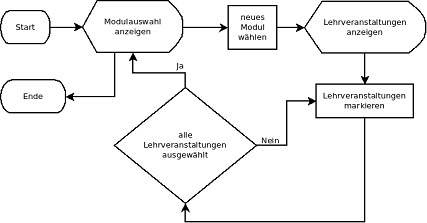
\includegraphics{img/flowchart.jpg}
\newpage

\section{Skeleton / Skelett}

\subsection{Paperprototype}

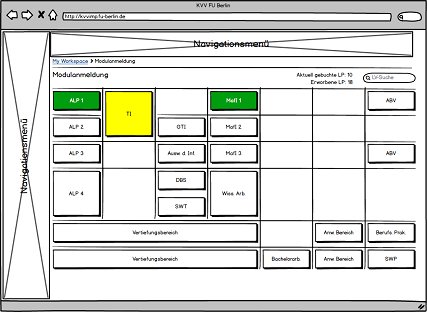
\includegraphics{img/ucd_ppt_start.png}\\
\\
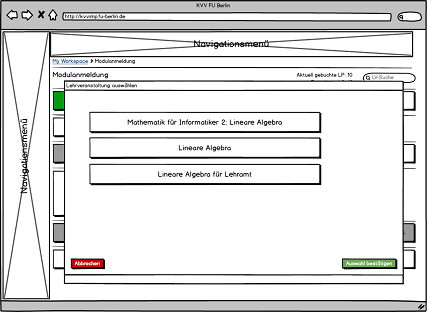
\includegraphics{img/ucd_ppt_lv_select.png}\\
\\
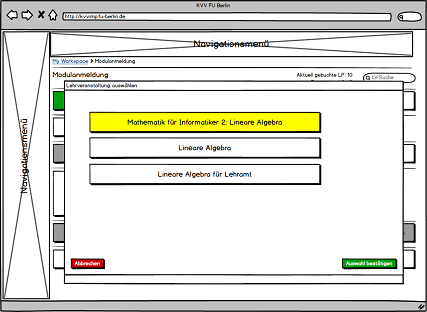
\includegraphics{img/ucd_ppt_lv_selected.png}\\
\\
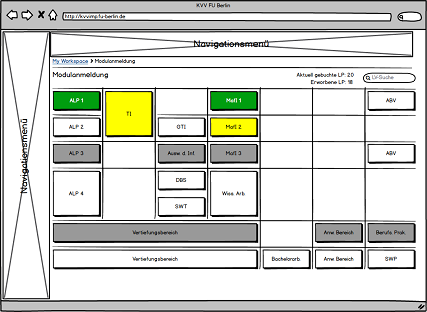
\includegraphics{img/ucd_ppt_mod_selected.png}\\
\\
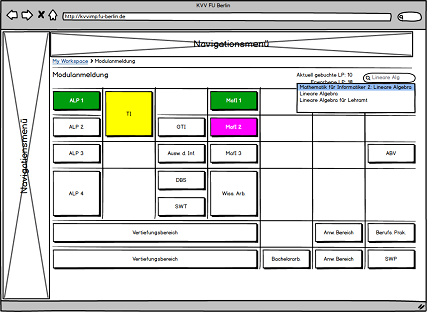
\includegraphics{img/ucd_ppt_lv_search.png}\\
\newpage

\subsection{Testszenario}

In einem Testszenario wird beschrieben wie der Paperprototype, bzw. eine Oberfläche, getestet werden soll. Im Falle des Paperprototypings nehmen am Test vier Personen teil:
\begin{itemize}
\item \textbf{Tester}\\
Diese Person testet den Paperprototype. Die testende Person bekommt eine Aufgabe übertragen, die sie mit Hilfe der präsentieren Oberfläche lösen soll. Der Tester spricht während des gesamten Tests fortlaufen vor sich hin (thinking aloud method).
\item \textbf{Moderator}\\
Diese Person erklärt dem Tester seine Aufgabe. Der moderierende Person kann während des Testdurchlauf unterstützend eingreifen, falls dieses unbedingt nötig wird.
\item \textbf{Computer}\\
Diese Person legt präsentiert abhängig von den Aktionen des Testers die entsprechenden Oberflächen.
\item \textbf{Observer}\\
Diese Person zeichnet alle Aktionen und Entscheidungen der testenden Person auf.
\end{itemize}
Für einen Test werden ein Moderatorskript (Moderator), ein Notizpapier (Observer) und der Paperprototype (Computer) benötigt.

\subsubsection{Testplan}

Der Testplan beschreibt welche Aktion die testende Person durchführen soll. Der Testperson wird lediglich die Aufgabe übertragen und keine bis wenig Hilfestellung beim Bearbeiten der Aufgabe gegeben.\\
\\
Aufgabe: Trage dich für das Modul MafI 2 ein.\\
\begin{tabular}{|r|l|}
\hline
Ziele / Ergebnisse & Benutzer hat das Modul MafI 2 gebucht.\\
\hline
Annahmen & Benutzer findet schnell das richtige Modul.\\
\hline
Schritte (Weg 1) & klickt auf MafI 2, markiert das Modul MafI 2, bestätigt Auswahl\\
Schritte (Weg 2) & sucht MafI 2, wählt MafI 2 aus den Suchergebnissen aus, bestätigt Auswahl\\
\hline
Zeitschätzung & 92 Sekunden (Ermittelt durch 3-Punkt-Schätzung\\
\hline
Hinweise & MafI 2 ist Lineare Algebra\\
\hline
Notizen & keine Notizen\\
\hline
\end{tabular}
\newpage

\subsubsection{Moderatorskript}

Der Moderator verwendet beim Testen einen Leitfaden um sicherzustellen, dass der Test korrekt durchgeführt wird:
\begin{enumerate}
\item Begrüßung
	\begin{itemize}
	\item Vorstellung der Teilnehmer
	\end{itemize}
\item Warm-up-Phase
	\begin{itemize}
	\item Icebreaker
	\item Nicht die Testperson wird getestet, sondern die Oberfläche.
	\end{itemize}
\item Präsentation der Aufgabe
	\begin{itemize}
	\item Erläuterung des Settings
	\item Erläuterung der Aufgabenstellung
	\end{itemize}
\item Durchführung
	\begin{itemize}
	\item Hinweis zur Verwendung der \textit{thinking aloud method}
	\item ergänzende Hilfestellung bei Fragen
	\end{itemize}
\item Verabschiedung
\end{enumerate}

\newpage

\section{Surface / Oberfläche}

\subsection{Heuristische Evaluation}

Die heuristische Evaluation ist ein ressourcenschonendes Mittel um benutzerunabhängig den Paperprototype oder eine Benutzeroberfläche systematisch auf Schwachstellen hin zu untersuchen. Hierfür wird ein best practice Regelwerk ausgewählt und abgearbeitet:\\
\\
\textbf{Antizipation}\\
\\
Im Suchfeld rechts oben wird bereits eine Autovervollständigung genutzt, die die passenden Module vorschlägt. Man könnte die Suche dadurch verbessern, in dem man auch Module in die Vorschlagsliste aufnimmt, die mit dem Suchbegriff assoziiert werden können.\\
\\
\textbf{Farbenblindheit}\\
\\
Die verwendeten Farben widersprechen der Heuristik für Farbenblindheit. Wir verwenden die Farben rot, gelb und grün als Ampelsystem. Diese Auswahl wurde allerdings bewusst getroffen.\\
\\
\textbf{Autonomie}\\
\\
Wir lassen dem Nutzer bestimmte Freiheiten, allerdings nur in dem Rahmen, der für den Nutzer sinnvoll ist. Er kann zum Beispiel nur diejenigen Module wählen, die in dem bestimmten Semester auch angeboten werden. Nicht wählbare Module werden ausgegraut.\\
\\
\textbf{Konsistenz}\\
\\
Wir verwenden das Corporate Design der Freien Universität. Die jeweiligen Screens sind vereinheitlicht. Die Programmierung erfolgt mit Wicket und lässt dem Entwickler trotzdem genug Freiheit.\\
\\
\textbf{Standartwerte}\\
\\
Man könnte einen Knopf anbieten, der eine automatisierte Modulbuchung gemäß Regelstudienplan umsetzt (pro Semester in dem sich der Studierende befindet). Da aus den Interviews der Wunsch nach einer individuellen Modulbuchung hervorging, sollte diese automatische Buchung ein zusätzliches Feature sein.\\
\\
\textbf{Fit's Law}\\
\\
Wurde berücksichtigt. An Stelle eines Home Buttons haben wir den My Workspace-Button. Der Abbrechen-Button ist immer an der gleichen Stelle. Wir haben allerdings kein X Knopf rechts oben in Kontextfenstern. Das war allerdings eine bewusste Entscheidung.\\
\\
\textbf{Effizenz des Nutzers}\\
\\
Es wurde bereits versucht, die Modulbuchung mit möglichst wenigen Arbeitsschritten umzusetzen. Die Anzahl der möglichen Funktionalitäten ist auf das wesentliche beschränkt.\\
\\
\textbf{Erforschbares Interface}\\
\\
Die Arbeitsschritte und Oberflächenkomponenten wurden auf das wesentliche reduziert (weniger ist mehr) und man kann einen Vorgang jederzeit abbrechen. Es gibt keine Shortcuts.\\
\\
\textbf{Lernbarkeit}\\
\\
Bei der Verarbeitung der Daten wird dem Nutzer angezeigt, welcher Arbeitsschritt momentan ausgeführt wird.\\
\\
\textbf{Metaphern}\\
\\
Die Suche wird durch eine Lupe repräsentiert.\\
\\
\textbf{Lesbarkeit}\\
\\
Es wird eine serifenfreie Schrift verwendet und Überschriften werden größer und dick gedruckt.\\
\\
\textbf{Trackstate}\\
\\
Da der Nutzer eingeloggt ist stehen uns alle Profilinformationen des Nutzers zur Verfügung.\\
\newpage

\subsection{Ergebnisse der heuristischen Evaluation}

Die folgende Auflistung ist nach der Wichtigkeit geordnet:\\
\textit{(sehr wichtig oben bis weniger wichtig unten)}
\begin{enumerate}
\item Anzeige von assoziierten Begriffen bei Suchergebnissen (Antizipation)
\item Modulübersicht muss gut lesbar dargestellt werden (Lesbarkeit)
\item Ampelprinzip als Anzeige für den Status eines Moduls (Farbenblindheit)
\item Einbinden von Shortcuts für schnelle Ausführung von Arbeitsschritten für erfahrene Benutzer (Erforschbares Interface)
\item Knopf \textit{automatische Buchung}, für die Modulbuchung gemäß Regelstudienplan (Standardwerte) 
\end{enumerate}
Mit Hilfe der Ergebnisse der heuristischen Evaluation wurde ein zweiter Paperprototype erzeugt und in einen High fidelity prototype umgesetzt.

\subsection{High fidelity prototype}

Im Folgenden ist der nach der Durchführung der heuristischen Evaluation aus dem zweiten Paperprototype entstandene High fidelity prototype zu sehen:\\
\\
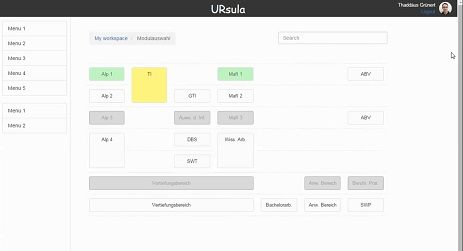
\includegraphics{img/hfp_v1}\\
\\
Dieser High fidelity prototype wurde überarbeitet, nachdem wir weitere Anregungen aus der Präsentation des Screencasts des ersten Prototypen erhielten.\\
\\
\\
\\
\\
\\
Die folgende Grafik enthält alle Änderungsanforderungen, die nach der erneuten Evaluierung entstanden.\\
\\
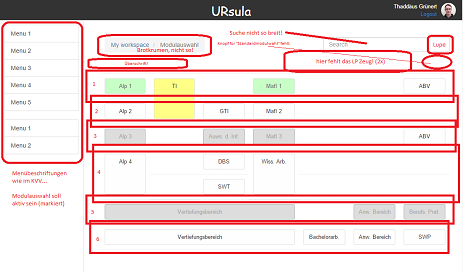
\includegraphics{img/hfp_changes}\\
\\
Abschließend ist das Endresultat des High fidelity prototypes zu sehen:
\\
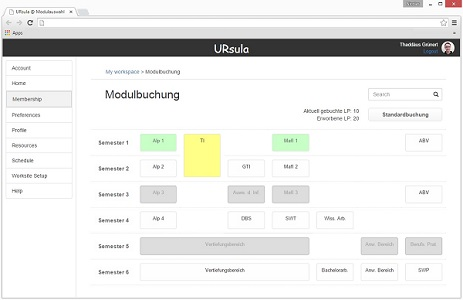
\includegraphics{img/prototype}\\
\newpage

\section{Anhang}

Der Anhang ist wie folgt strukturiert:
\begin{enumerate}
\item Persona; Seite 27
\item Primary Nouns für das LMS; Seite 28
\item Zweite überarbeitete Version des Paperprototypes; Seiten 29,30,31,32,33
\end{enumerate}

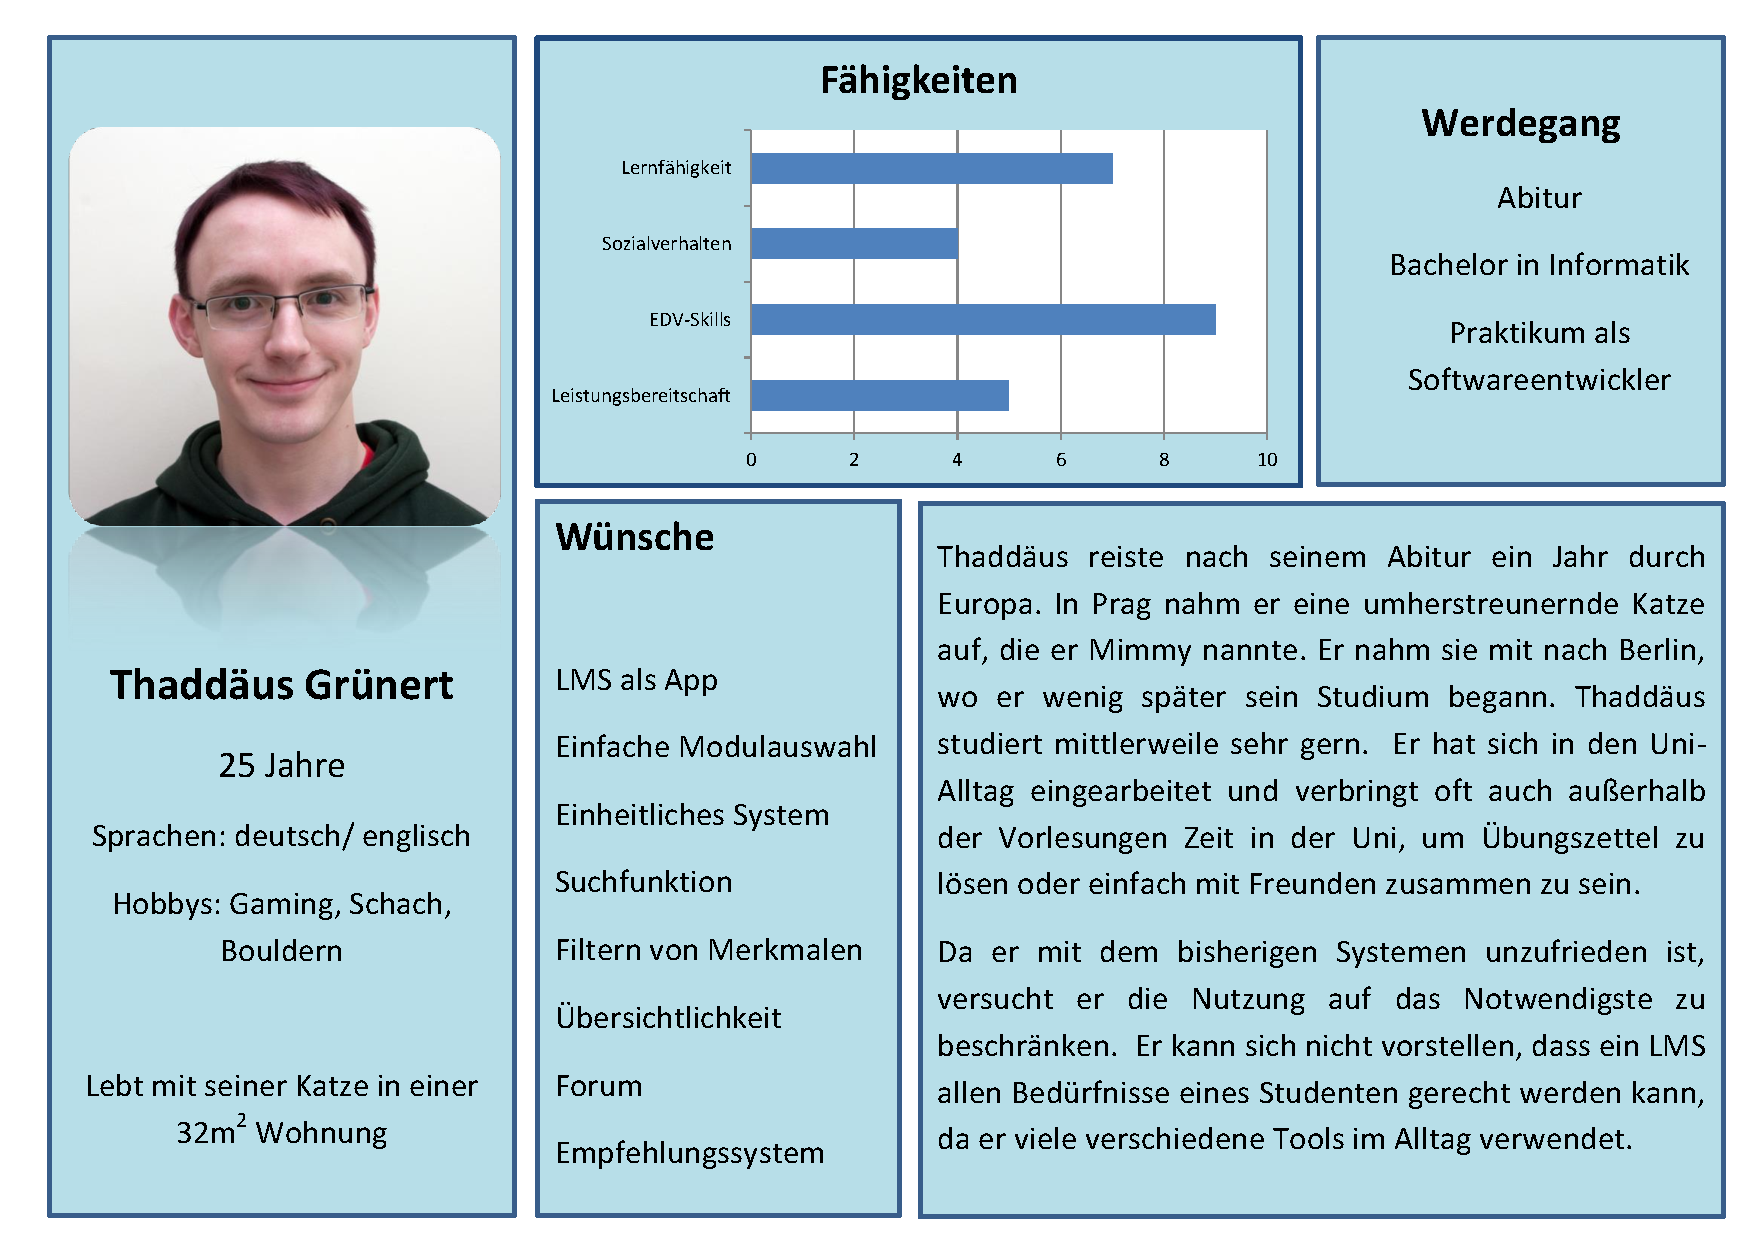
\includepdf[landscape]{include/persona.pdf} 
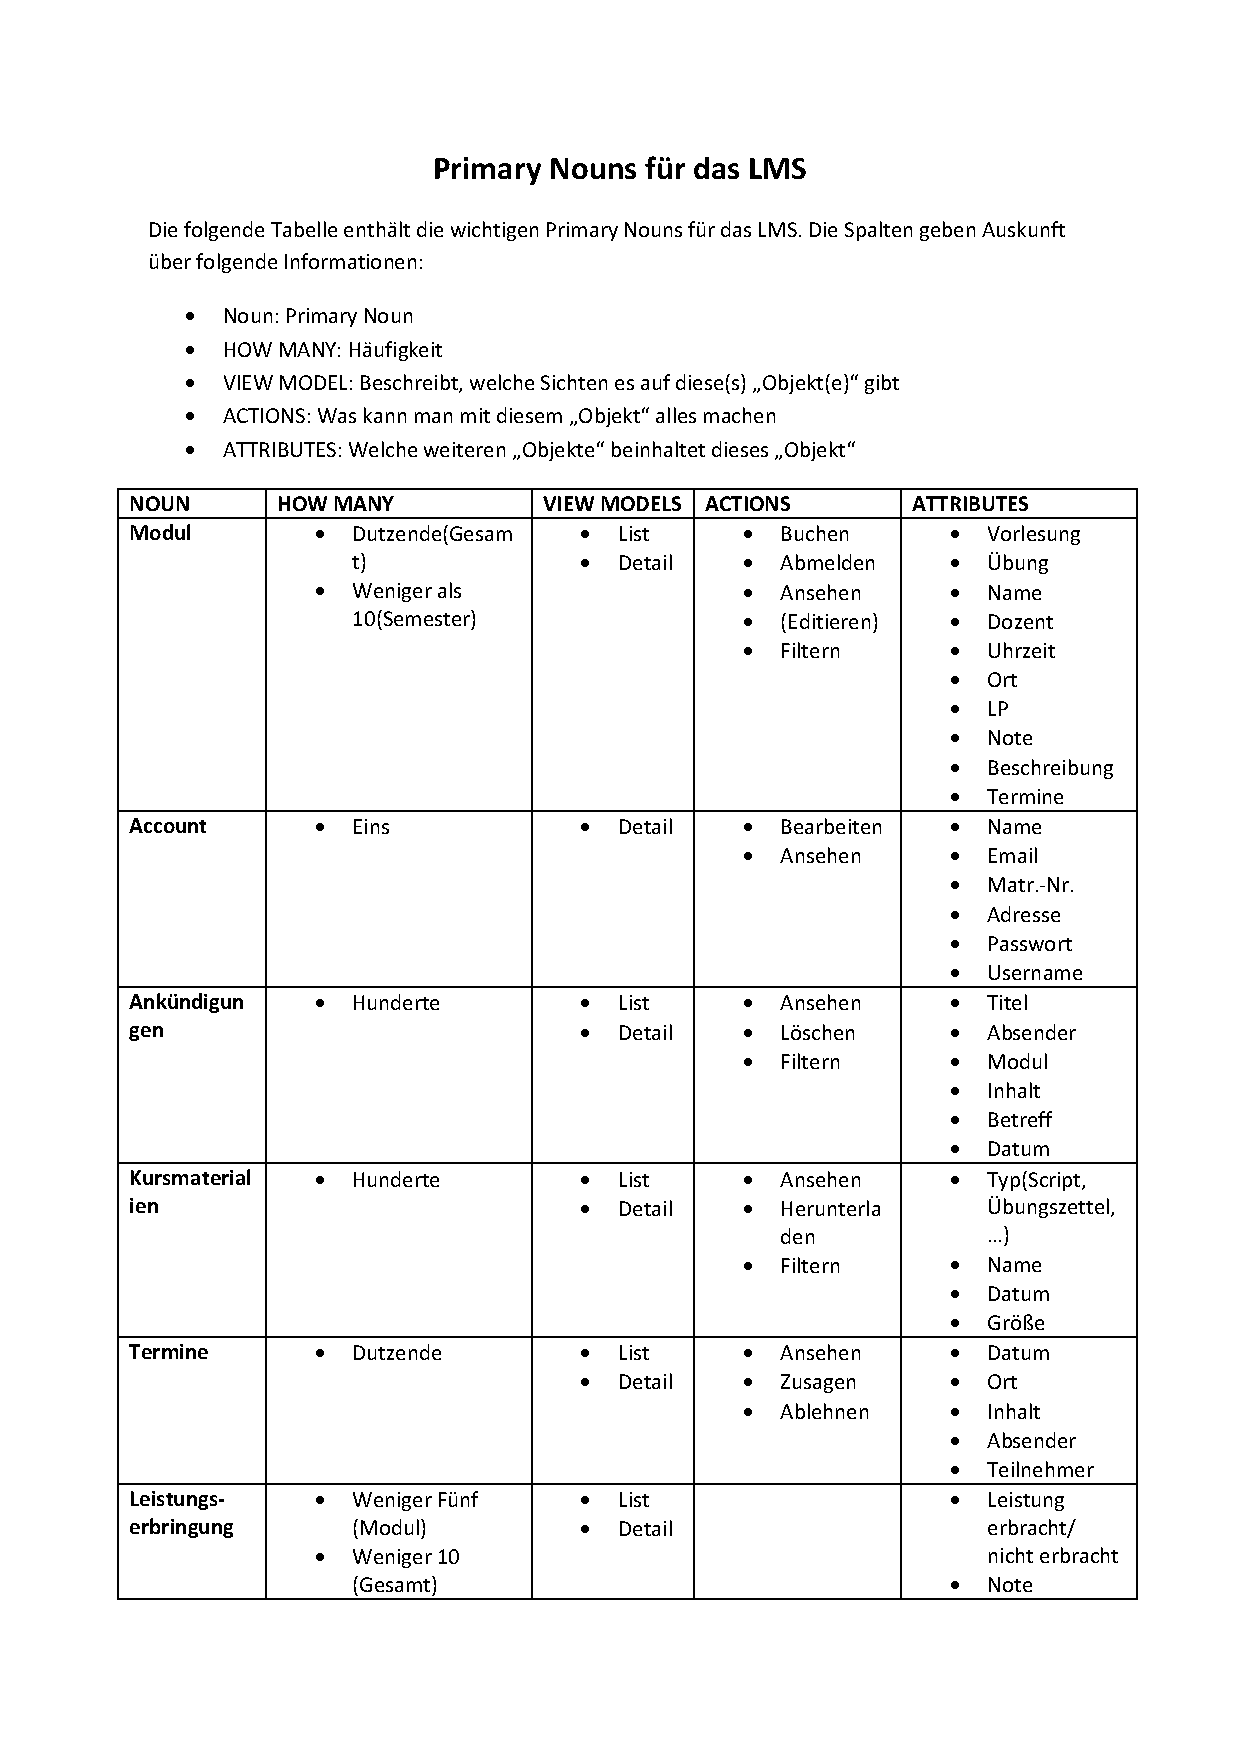
\includepdf{include/pnoun.pdf}
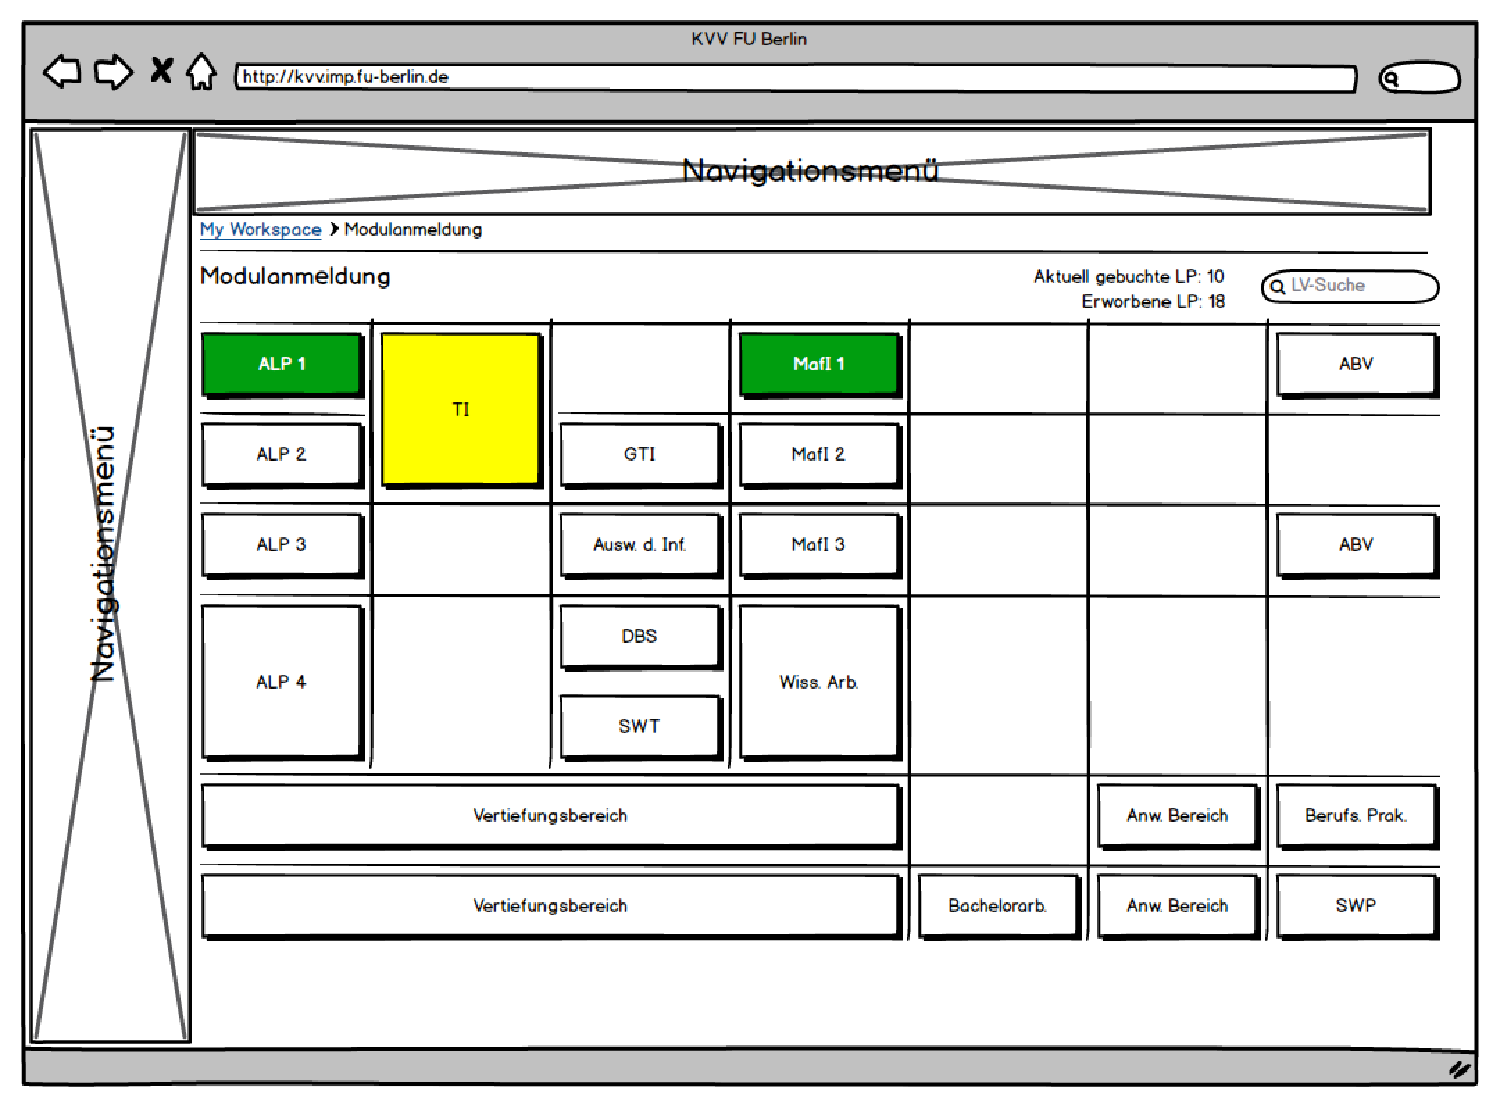
\includepdf[landscape,pages={1,2,3,4,5}]{include/ppt.pdf}
\end{document}